% !TEX root = ../thesis.tex
% basics
% @author Tobias Wulf
%

\chapter{Grundlagen 0.0.2 19.02.2021}\label{ch:grundlagen}

Das Fundament für die Drehwinkelerfassung mittels magnetischen Sensor-Array und lernender Signalverarbeitung 
\cite{Schuethe2019}\cite{Schuethe2020a}\cite{Schuethe2020}, die auf Regressionsverfahren für Gauß-Prozesse 
\cite{Rasmussen2006} aufbauen, bildet sich durch Abstandmessungen von Winkelpositionen auf einer Kreisbahn. Für eine
anschauliche Erklärung der Zusammenhänge soll als Einstieg in die Grundlagen, das Prinzip anhand eindimensionaler 
Vektorfelder zweier Winkelstellungen $A$ und $B$ gezeigt werden. Das entspräche einem Anwendungsfall einfacher und 
heute erhältlicher magnetischer Sensoren, wie dem KMZ60 \cite{NXPSemiconductors2014} von NXP, oder dem  TAS2141-AAAB 
\cite{TDK2016} der Firma TDK. Die Verfahrensgrundlage, der eindimensionalen Betrachtung, wird in der Verwendung von 
Sensor-Arrays adaptiert und durch geeignete Rechen- und Normierungsverfahren auf die Problemstellung eines 
höherdimensionalen Systems projiziert.


Der in \autoref{fig:veranschaulichung-sensor-ic} gezeigte Anwendungsfall, soll hier als Grundlage der Erläuterungen 
dienen. Genaue technische und physikalische Größenzusammenhänge sind vorerst vernachlässigt. 
\autoref{fig:veranschaulichung-sensor-ic} zeigt eine kreisförmige Rotation des Gebermagneten um seine $Z$-Achse. 
Entsprechend rotiert das Magnetfeld bei Drehung des Magneten mit. Der darunter liegende Sensor erfasst die 
Magnetfeldstärke $\vec{H}$ des Gebermagnetfeldes. Die Winkelstellung $\alpha$ des Magneten kann dabei nicht direkt 
erfasst werden. Der Sensor misst, die zueinander und zur Rotationsachse orthogonal stehenden, $X$- und $Y$-Komponenten 
der Gebermagnetfeldstärke $\vec{H}$ und setzt diese in elektrische Spannungssignale um. Bedingt durch die Kreisbewegung 
und Orthogonalität, lässt sich die Winkelstellung mittels einfacher Vektorrechnung bestimmen. 


\clearpage


Bei idealer und gleichbleibender Position des Magneten in Relation zum Sensor, beschreiben die aufgenommen Messpunkte 
eine Kreisbahn mit konstanten Bahnradius $r$ und Winkelstellung $\alpha$ des Gebermagneten. 
\autoref{fig:kreisdarstellungwinkelabstand} zeigt den Zusammenhang für zwei erfasste Winkelstellungen $A$ und $B$. Es 
ergeben sich für die beiden Winkelstellungen $A\mapsto\alpha_1$ und $B\mapsto\alpha_2$ folgende vektorielle 
Zusammenhänge in \autoref{eq:vektorenab}.


\begin{equation}\label{eq:vektorenab}
\begin{aligned}
	A &= 
		\begin{pmatrix} 
			a_x \\
			a_y 
		\end{pmatrix}
	  &= 
		\begin{pmatrix} 
			r \cdot \cos(\alpha_1) \\
			r \cdot \sin(\alpha_1) 
		\end{pmatrix} \\
	B &=
		\begin{pmatrix} 
			b_x \\
			b_y 
		\end{pmatrix}
	  &= 
		\begin{pmatrix} 
			r \cdot \cos(\alpha_2) \\
			r \cdot \sin(\alpha_2) 
		\end{pmatrix} \\
\end{aligned}
\end{equation}


Die vom Sensor erfassten und umgewandelten $X$- und $Y$-Komponenten der Messpunkte $A$ oder $B$, bilden 
eindimensionale Vektorfelder. Über ihren Betrag lässt sich der Bahnradius $r$ ermitteln, zu sehen in 
\autoref{eq:vektor2norm}. Allgemein ist der Betrag eines Vektors über die Vektor-2-Norm zu berechnen. Diese Norm 
wird oft auch als euklidische Norm bezeichnet.


\begin{equation}\label{eq:vektor2norm}
	\begin{aligned}
	r &:= &\|A\|_2 &= &\sqrt{\sum_{i=1}^{n}|A_i|^2} &= &\sqrt{|a_x|^2 + |a_y|^2} &= &|A| &= &konst. \\
	  &&&&&\equiv \\
	  &   &\|B\|_2 &= &\sqrt{\sum_{i=1}^{n}|B_i|^2} &= &\sqrt{|b_x|^2 + |b_y|^2} &= &|B| &= &konst.
	\end{aligned}
\end{equation}


Der direkte Winkelabstand zwischen $A$ und $B$ kann geometrisch, wie in \autoref{fig:kreisdarstellungwinkelabstand} 
gezeigt, über die Abstandsquadrate der vektoriellen Anteile ermittelt werden und ist gleich der Kantenlänge des 
Quadrates zwischen den Punkten $A$ und $B$. Entsprechend der Kreisbahnnormierung für die Messpunkte, ist diese Form der 
Abstandsermittlung als euklidischer Abstand $d_E\langle A,B \rangle$ bezeichnet. Zu berechnen ist der Abstand 
$d_E\langle A,B \rangle$ nach \autoref{eq:euklidischerabstand} als Vektor-2-Norm der vektoriellen Differenz von $A$ und 
$B$.


\begin{equation}\label{eq:euklidischerabstand}
	d_E\langle A,B \rangle = \|A - B\|_2 = \sqrt{\sum_{i=1}^{n}(A_i - B_i)^2} = \sqrt{(a_x - b_x)^2 + (a_y - b_y)^2}
\end{equation}


\clearpage


Für den euklidischen Abstand zwischen zwei Winkelstellungen $d_E\langle A,B \rangle$ und das Quadrat des Abstandes 
$d_E^2\langle A,B \rangle$ muss die Dreiecksungleichung nach \autoref{eq:v2ndreiecksungleichung} für allgemeine 
Vektor-2-Normen gelten \cite{vandeGeijn2014}. Dieser Zusammenhang kann genutzt werden um eine Kreisbahn zu 
approximieren, wenn der Bahnradius $r$ nicht konstant und $\|A\|_2 \ne \|B\|_2$ ist. 


\begin{equation}\label{eq:v2ndreiecksungleichung}
	\begin{gathered}
	\big|\|A\|_2 - \|B\|_2\big| \le \|A \pm B\|_2 \le \big|\|A\|_2 + \|B\|_2\big| \\
	\Downarrow \\
	\big(\|A\|_2 - \|B\|_2\big)^2 \le \|A - B\|_2^2 = d_E^2\langle A,B \rangle
	\end{gathered}
\end{equation}


\begin{figure}[tbph]
	\centering
	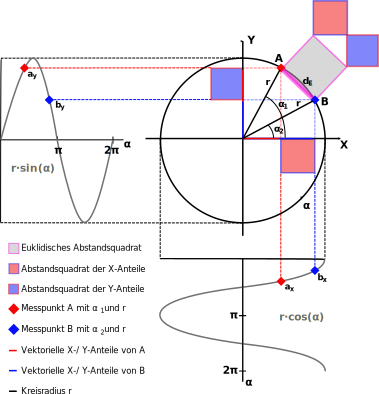
\includegraphics[width=0.7\linewidth]{chapters/images/Kreisdarstellung_Winkelabstand}
	\caption[Allg. Kreisdarstellung des euklidischen Winkelabstands]{Allg. Kreisdarstellung des euklidischen 
	Winkelabstands. Die Kreisdarstellung zeigt den euklidischen Winkelabstand zweier Winkelmesspunkte $A$ und $B$ 
	mit gleichen Kreisradius $r$. Der euklidische Abstand, bzw. das Abstandsquadrat, zwischen den Winkelposition 
	$A$ und	$B$ ist zerlegt in Abstandsquadratanteile. Die Abstandquadratanteile ergeben sich aus der vektoriellen 
	Zusammensetzung in $X$-/ $Y$-Anteile für die einzelnen Messpunkte $A$ und $B$.}
	\label{fig:kreisdarstellungwinkelabstand}
\end{figure}


\clearpage


Bei konstant bleibenden Bahnradius $r$ befindet sich der Abstand $d_E\langle A,B \rangle$ im Intervall $0 \le 
d_E\langle A,B \rangle \le \sqrt{2}\cdot r$. Die Winkelstellungen des Gebermagnet lassen sich über die Vektoranteile 
der Messpunkte und den Bahnradius $r$ berechnen. Also eine Überführung aus kartesischer Darstellung der Messpunkte in 
ihre Polarkoordinaten aus \autoref{eq:vektorenab}. Hier in \autoref{eq:umrechnungpolar} für beliebige Messpunkte auf 
der Kreisbahn gezeigt.

\begin{equation}\label{eq:umrechnungpolar}
	\cos(\alpha) = \frac{x}{r} \quad\sin(\alpha) = \frac{y}{r} \quad\tan(\alpha) = \frac{y}{x}
\end{equation}

\begin{equation}
	\alpha' = 
	\begin{cases}
		+\arccos\left(\frac{x}{r}\right)        & \quad\text{f. } \arcsin\left(\frac{y}{r}\right) \ge 0\\
		-\arccos\left(\frac{x}{r}\right) + 2\pi & \quad\text{f. } \arcsin\left(\frac{y}{r}\right) < 0
	\end{cases}
\end{equation}


\begin{figure}[tbph]
	\centering
	\includegraphics[width=0.5\linewidth]{chapters/images/Winkelumrechnung_Polar}
	\caption[Winkelrückrechnung mit Bereichsumschaltung]{Winkelberechnung mit Bereichsumschaltung. Die Berechnung des 
	Winkel $\alpha'$ erfolgt über die $\arccos$ und $\arcsin$ Funktion, bzw. die vektoriellen Anteile der Messpunkte. 
	Die $\arcsin$ Funktion bildet dabei den Schwellwert für die Bereichsumschaltung um eine volle Rotation abzubilden.}
	\label{fig:winkelumrechnungpolar}
\end{figure}



\begin{itemize}
	\item Einleitung Aufgabenfeld
	\item Einheitskreis
	\item Bezug zur Drehwinkelerfassung und Sensorapplikation
\end{itemize}
\clearpage


\section{Magnetische Sensorentypen und mechatronische Anwendung}\label{sec:magnetische-sensorentypen}
	\begin{itemize}
		\item Die Technologie mit der ein Sensorkopf realisiert ist, klassifiziert in der Regel die Sensorbezeichnung. Anhänge in der Bezeichnung wie AMR oder TMR, geben somit Auskunft darüber welche Technologie für die Realisierung des Sensorkopfes die Grundlage bildet.
		\item Anwendungsfall Winkelmessung
		\item Aufbau Sensorbrücke TMR (Umriss aus Datenblatt)
		\item Ausblick TMR Drehzahlmessung und Strommessung
	\end{itemize}

Die Konzipierung magnetischer Sensoren für die Drehwinkelerfassung richtet sich auf die Erfassung eines kreisförmigen 
Anregungsmagnetfeldes mit einer Feldstärke $\vec{H}$. Also ein kreisförmig rotierendes Magnetfeld, zumeist erzeugt 
durch einfache zweipolige Gebermagneten. Die räumliche Anordnung der Anwendung ist in 
\autoref{fig:veranschaulichung-sensor-ic} zu sehen. Das Magnetfeld rotiert um die $Z$-Achse des Sensors. Zur Detektion 
des Magnetfeldes bzw. seiner Rotation sind dessen Anteile in $X$- und $Y$-Richtung genutzt. Die Nord-Südausrichtung des 
Gebermagneten liegt dabei in der $X$- bzw. $Y$-Achse der Anwendung, bestehend aus Magnet und Sensor. Die Magnetfeldst 
des Gebermagneten ist durch seine vektoriellen Anteile in $X$, $Y$ und $Z$-Richtung beschrieben \cite{Pape2017}. Weitere

\begin{equation}\label{eq:hfeldanteile}
\vec{H} = \begin{pmatrix}H_x\\H_y\\H_z\end{pmatrix}
\end{equation}

Die Einheit der Feldstärke $\vec{H}$ ist $\SI{}{\ampere\per\metre}$. Gängige Feldstärkengrößen für eine magnetische 
Anregung von Drehwinkelsensoren liegen Bereich $\SI{}{\kilo\ampere\per\metre}$.

\begin{figure}[tbph]
	\centering
	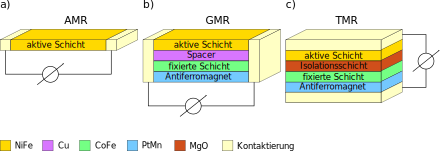
\includegraphics[width=\linewidth]{chapters/images/MR_Schichtmodelle}
	\caption[Schichtmodelle dreier magnetoresistive Effekte]{Schichtmodelle dreier magnetoresistive Effekte. a) 
	\gls{gl:amr}, schwache Widerstandsänderung. b) \gls{gl:gmr} stärkere Widerstandsänderung. c) \gls{gl:tmr} stärkste 
	Widerstandsänderung. Grafik entnommen aus \cite{Lemme2016}.}
	\label{fig:mrschichtmodelle}
\end{figure}



\begin{figure}[tbph]
	\centering
	\includegraphics[width=\linewidth]{chapters/images/TMR_Drehwinkelapplikation}
	\caption[TMR Drehwinkelapplikation]{TMR Drehwinkelapplikation. Schematisch gezeigt für eine volle Rotation des 
	Gebermagneten um $\SI{360}{\degree}$. Zu sehen sind die um $\SI{90}{\degree}$ verdrehten Wheatstone-Brücken des 
	Sensors. Die Brücken bilden, bei rotierenden Gebermagnetfeld, eine Sinus- und Cosinus-Funktion nach. Die Pfeile in 
	den einzelnen Widerständen weisen auf ihre magnetische Ausrichtung hin. Grafik entnommen und bearbeitet aus 
	\cite{Schuethe2020a}.}
	\label{fig:tmrdrehwinkelapplikation}
\end{figure}


\clearpage


\section{Kennfeldmethode zur Charakterisierung von Sensoren}\label{sec:kennfeldmethode-zur-charakterisierung}
	\begin{itemize}
		\item Überleitung von Sensorbrückenschaltung
		\item Messprinzip für das Erstellen der Sensorbrücken-Kennfelder
		\item Festlegung von Arbeitsbereich (Plateau TMR), Sättigung (KMZ60)
		\item Dimensionierung des Stimulus, Dipole Anregung
	\end{itemize}
	
	
	\clearpage
	\begin{figure}[tbph]
		\centering
		\includegraphics[width=\linewidth]{chapters/images/Magnetfeldstimulus_Kennfeldmethode}
		\caption[Magnetfeldstimulus zur Erzeugung von Sensorkennfeldern]{Magnetfeldstimulus zur Erzeugung von 
		Sensorkennfeldern. Es sind die Bestandteile des magnetischen Sensorstimuli dargestellt, die zum Ausmessen des 
		Sensorkennfeldes in $H_x$- und $H_y$-Richtung verwendet worden sind. Es ist das Prinzip des Verfahrens 
		dargestellt. In a) und b) ist die Dreiecksmodulation des magnetischen Anregungsfeldes abgebildet. Für a) die 
		$H_x$-Feldanregung mit Cosinus-Trägerwelle und für b) die $H_y$-Feldanregung mit Sinus-Trägerwelle. Es sind für 
		beide Anregungsrichtungen niedrige Frequenzen gewählt um ein quasi-statisches Anregungsmagnetfeld zu erzeugen. 
		Es ergeben sich für die Betragsamplitude des Stimulus, in polarer Darstellung c) und d), konzentrische 
		Trajektorien. Diese verlaufen von Innen nach Außen für die steigende Flanke der Amplitudenmodulation c) und von 
		Außen nach Innen für die fallende Flanke d). Die Dreieckmodulationsfrequenz liegt bei $f_m = \SI{0.1}{\hertz}$ 
		und einer Trägerwellenfrequenz $f_c = \SI{3.2}{\hertz}$. Grafik nachempfunden aus \cite{Schuethe2019}.}
		\label{fig:magnetfeldstimuluskennfeldmethode}
	\end{figure}
	
	
	\clearpage
	\begin{figure}
		\centering
		\includegraphics[width=\linewidth]{chapters/images/TDK_Kennfelder}
		\caption[TDK TAS2141-AAAB Winkelsensorbrückenkennfelder]{TDK TAS2141-AAAB Winkelsensorbrückenkennfelder. Zu 
		sehen sind die Kennfelder der Cosinus-Brücke a) und b). Darunter befinden sich die Kennfelder der Sinus-Brücke 
		c) und d). Die Kennfelder für beide Brücken a) und c) beziehen sich auf die steigenden Flanke der 
		Amplitudenmodulation aus \autoref{fig:magnetfeldstimuluskennfeldmethode} und die in b) bzw. d) gezeigten 
		Kennfelder sind gewonnen aus der fallenden Flanke. Die Brückenkennfelder sind normiert in 
		$\SI{}{\milli\volt\per\volt}$. Für eine Spannungsausgabe in Betriebsspannungsniveau ist keine zusätzliche 
		Verstärkung notwendig. Die Kennfelder besitzen, jeweils in $H_x$- und $H_y$-Richtung, eine Schrittweite von 
		$\SI{0.1961}{\kilo\ampere\per\metre}$ und sind skaliert von $\SI{-25}{\kilo\ampere\per\metre}$ bis 
		$\SI{+25}{\kilo\ampere\per\metre}$. Somit ergibt sich eine Bildauflösung für ein Kennfeld von $256 \times 256$ 
		Messpunkten. Grafik nachempfunden aus \cite{Schuethe2019}.}
		\label{fig:tdkkennfelder}
	\end{figure}
	
	
	\clearpage
	\begin{figure}[tbph]
		\centering
		\includegraphics[width=\linewidth]{chapters/images/KMZ60_Kennfelder}
		\caption[NXP KMZ60 Winkelsensorbrückenkennfelder]{NXP KMZ60 Winkelsensorbrückenkennfelder. Zu sehen sind die 
		Kennfelder der Cosinus-Brücke a) und b). Darunter befinden sich die Kennfelder der Sinus-Brücke c) und d). 
		Die Kennfelder für beide Brücken a) und c) beziehen sich auf die steigenden Flanke der Amplitudenmodulation aus 
		\autoref{fig:magnetfeldstimuluskennfeldmethode} und die in b) bzw. d) gezeigten Kennfelder sind gewonnen aus 
		der fallenden Flanke. Die Brückenkennfelder sind normiert in $\SI{}{\milli\volt\per\volt}$. Für eine 
		Spannungsausgabe in Betriebsspannungsniveau ist eine zusätzliche Verstärkung um Faktor $42$ notwendig. Die 
		Kennfelder besitzen, jeweils in $H_x$- und $H_y$-Richtung, eine Schrittweite von 
		$\SI{0.1961}{\kilo\ampere\per\metre}$ und sind skaliert von $\SI{-25}{\kilo\ampere\per\metre}$ bis 
		$\SI{+25}{\kilo\ampere\per\metre}$. Somit ergibt sich eine Bildauflösung für ein Kennfeld von $256 \times 256$ 
		Messpunkten. Grafik nachempfunden aus \cite{Schuethe2019}.}
		\label{fig:kmz60kennfelder}
	\end{figure}
	
	
	\clearpage
	\begin{figure}[tbph]
		\centering
		\includegraphics[width=\linewidth]{chapters/images/TDK_Kennfeld_Steigend}
		\caption[TDK TAS2141-AAAB Kennfeldquerschnitte]{TDK TAS2141-AAAB Kennfeldquerschnitte. Für die Kennfelder 
		gewonnen aus steigender Amplitudenmodulation a) und c). Es sind Querschnitte durch die jeweiligen Kennfelder in 
		b) und d)abgebildet. Für $V_{cos}$ a), b) verschiedene konstante $H_y$ und $V_{sin}$ c), d) entsprechend 
		verschiedene konstante $H_x$ Querschnitte. Grafik nachempfunden aus \cite{Schuethe2019}.}
		\label{fig:tdkkennfeldsteigend}
	\end{figure}
	
	
	\clearpage
	\begin{figure}[tbph]
		\centering
		\includegraphics[width=\linewidth]{chapters/images/KMZ60_Kennfeld_Steigend}
		\caption[NXP KMZ60 Kennfeldquerschnitte]{NXP KMZ60 Kennfeldquerschnitte. Für die Kennfelder gewonnen aus 
		steigender Amplitudenmodulation a) und c). Es sind Querschnitte durch die jeweiligen Kennfelder in b) und d) 
		abgebildet. Für $V_{cos}$ a), b) verschiedene konstante $H_y$ und $V_{sin}$ c), d) entsprechend verschiedene 
		konstante $H_x$ Querschnitte. Grafik nachempfunden aus \cite{Schuethe2019}.}
		\label{fig:kmz60kennfeldsteigend}
	\end{figure}
	
	
	\clearpage
	\begin{figure}[tbph]
		\centering
		\includegraphics[width=\linewidth]{chapters/images/TDK_Uebertragungskennlinien}
		\caption[TDK TAS2141-AAAB Übertragungskennlinie]{TDK TAS2141-AAAB Übertragungskennlinie. Es sind wieder die 
		Kennfelder aus der steigenden Amplitudenmodulation in a) und b). In c) sind die Übertragungskennlinien für den 
		Sensor gezeigt mit Kennzeichnung für den Betrieb auf dem linearen Plateau des Kennfeldes bei 
		$\SI{8.5}{\kilo\ampere\per\metre}$. Ebenfalls zu sehen in a) und b) durch die sich ergebene Kreisbahn mit einem 
		Radius des aufgelegten Intervalls aus c). Grafik nachempfunden aus \cite{Schuethe2019}.}
		\label{fig:TDKuebertragungskennlinien}
	\end{figure}

	
	\clearpage
	\begin{figure}[tbph]
		\centering
		\includegraphics[width=\linewidth]{chapters/images/KMZ60_Uebertragungskennlinien}
		\caption[NXP KMZ60 Übertragungskennlinie]{NXP KMZ60 Übertragungskennlinie. Es sind wieder die Kennfelder aus 
		der steigenden Amplitudenmodulation in a) und b). In c) sind die Übertragungskennlinien für den Sensor gezeigt 
		mit Kennzeichnung für den Betrieb in Sättigung bei $\SI{20}{\kilo\ampere\per\metre}$. Ebenfalls zu sehen in a) 
		und b) durch die sich ergebene Kreisbahn mit einem Radius des aufgelegten Intervalls aus c). Grafik 
		nachempfunden aus \cite{Schuethe2019}.}
		\label{fig:kmz60uebertragungskennlinien}
	\end{figure}

	
	\clearpage
	\begin{figure}[tbph]
		\centering
		\includegraphics[width=\linewidth]{chapters/images/Approximierter_Kugelmagnet}
		\caption[Approximierter Kugelmagnet]{Approximierter Kugelmagnet. Die Approximation des Kugelmagneten erfolgt 
		über Dipol-Feldgleichung in Näherung des Kugelmagnetfernfeldes. Das Magnetfeld ist auf 
		$\SI{200}{\kilo\ampere\per\metre}$ bei einem Abstand von $\SI{1}{\milli\metre}$ zur Kugelmagnetoberfläche 
		normiert. Der Radius des Kugelmagneten beträgt $\SI{2}{\milli\metre}$.}
		\label{fig:dipolemagnet}
	\end{figure}
	
	
	\clearpage
	
	
\section{Prinzip des Sensor-Arrays}\label{sec:prinzip-des-sensor-arrays}
	\begin{itemize}
		\item geometrischer Aufbau
		\item Brückenausgangsspannungen
		\item Resultierende Array-Datenformate und Darstellung der Sinoiden
	\end{itemize}

\section{Sensor-Array-Simulation über Dipol-Feldgleichung}\label{sec:sensor-array-simulation-dipol-feldgleichung}
	\begin{itemize}
		\item Erzeugen des Meshgrids
		\item Normieren des Magnetfeldes
		\item Erzeugen von Rotationsmomenten (inkl. Verkippung)
		\item Referenzierung zu Kennfeldern und Gewinnung der Brückenspannungen (interp2 nearest neighbor)
	\end{itemize}

\section{Gauß-Prozesse für Regressionsverfahren}\label{sec:gauss-prozesse-regressionsverfahren}
	\begin{itemize}
		\item Erläuterung des Regressionsverfahren im allg.
		\item Bedeutung und Kriterien der Kovarianzfunktion, Spiegel der Applikation
		\item Herleitung der Quadratischen Frobenius Kovarianzfunktion mit Bezug zum Einheitskreis
		\item Möglichkeiten zur Mittelwertschätzung und -Korrektur
		\item Optimierungskriterien in der Trainingsphase
		\item Qualitätskriterien in der Arbeitsphase
	\end{itemize}